\documentclass[tikz,border=4pt]{standalone}

\usepackage{lmodern}
\usepackage{amsmath,amssymb}
\usetikzlibrary{arrows.meta,calc,positioning}

\definecolor{Ink}{HTML}{1E2830}
\definecolor{Muted}{HTML}{66727C}
\definecolor{LineGray}{HTML}{CAD2D9}
\definecolor{Blue}{HTML}{246BB2}
\definecolor{Navy}{HTML}{133F78}
\definecolor{PaleBlue}{HTML}{F2F7FC}
\definecolor{Orange}{HTML}{E9860A}
\definecolor{Purple}{HTML}{7C3DA4}
\definecolor{PalePurple}{HTML}{FAF7FC}
\definecolor{Green}{HTML}{2D7C37}
\definecolor{PaleGreen}{HTML}{F5FAF5}
\definecolor{Red}{HTML}{C9473E}

\tikzset{
  flow/.style={-{Latex[length=2.5mm,width=2mm]},draw=Blue,line width=.75pt},
  grayflow/.style={-{Latex[length=2.8mm,width=2.2mm]},draw=LineGray,line width=1.8pt},
  greenflow/.style={-{Latex[length=2.5mm,width=2mm]},draw=Green,line width=.8pt},
  panelblue/.style={draw=Blue!70,line width=.75pt,rounded corners=4pt,fill=white},
  panelpurple/.style={draw=Purple,line width=.8pt,rounded corners=4pt,fill=PalePurple},
  panelgreen/.style={draw=Green,line width=.8pt,rounded corners=4pt,fill=PaleGreen},
  task/.style={draw=Blue!72,line width=.65pt,rounded corners=3pt,fill=PaleBlue,
    align=center,text=Ink,font=\fontsize{11.2}{13.2}\selectfont},
  result/.style={draw=Purple!75,line width=.7pt,rounded corners=3pt,fill=white,
    align=center,text=Ink,font=\fontsize{11.2}{13.2}\selectfont},
  verify/.style={draw=Green!78,line width=.7pt,rounded corners=3pt,fill=white,
    align=left,text=Ink,font=\fontsize{11.2}{13.2}\selectfont},
  roundtag/.style={draw=Blue,rounded corners=2pt,inner xsep=5pt,inner ysep=2.5pt,
    font=\fontsize{13.5}{15}\selectfont\bfseries,text=Navy,fill=white},
}

\newcommand{\PIbadge}[2]{%
  \node[draw=Orange,fill=Orange!6,rounded corners=1.5pt,inner xsep=4pt,inner ysep=2.5pt,
        font=\fontsize{10.5}{11.5}\selectfont\bfseries,text=Ink] at (#1,#2) {PI};%
}

\newcommand{\Sbadge}[3]{%
  \node[circle,draw=Blue,line width=.75pt,fill=white,minimum size=.80cm,inner sep=0pt,
        font=\fontsize{10.5}{11.5}\selectfont\bfseries,text=Navy] at (#1,#2) {#3};%
}

\newcommand{\acceptbadge}[2]{%
  \node[draw=Green,fill=white,rounded corners=1.5pt,inner xsep=5pt,inner ysep=2.5pt,
        font=\fontsize{10.5}{11.5}\selectfont\bfseries,text=Green] at (#1,#2) {ACCEPT};%
}

\begin{document}
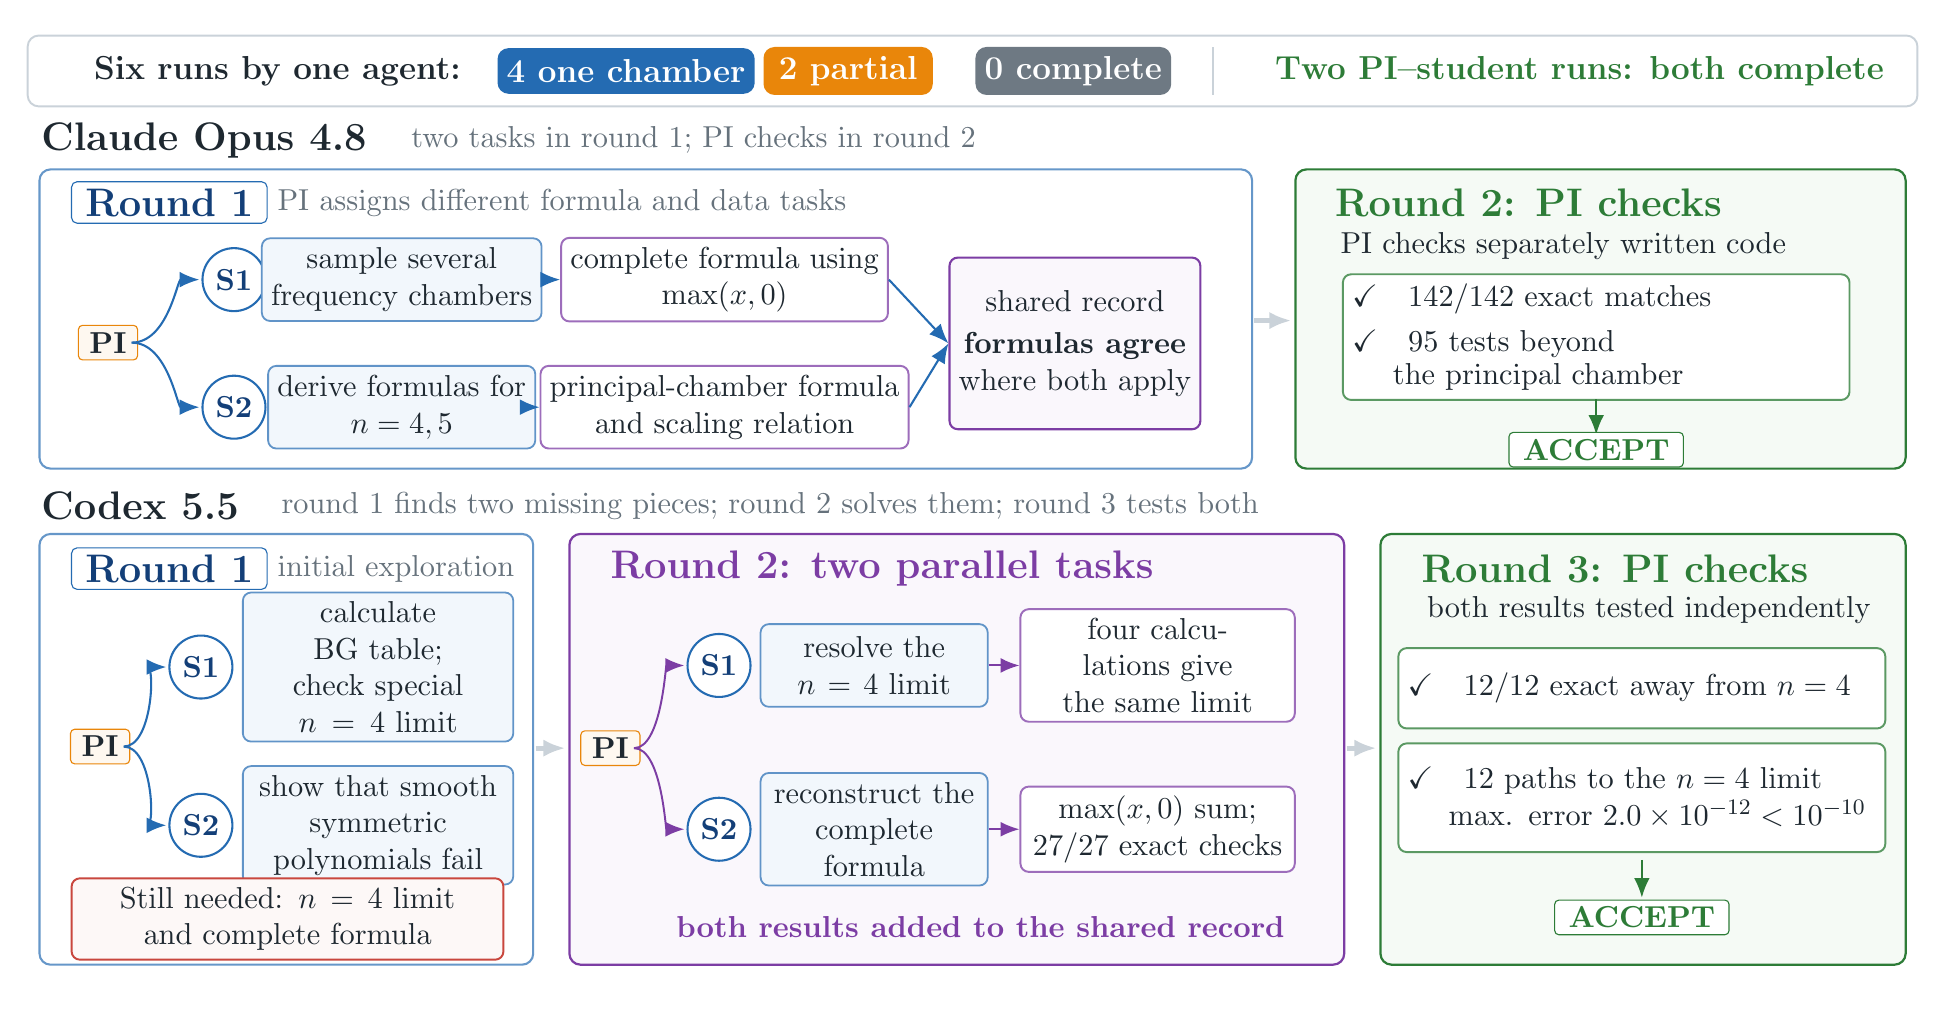
\begin{tikzpicture}[x=1cm,y=1cm]
  \path[use as bounding box] (0,0) rectangle (24,12.15);

  % Compact outcome context.
  \draw[draw=LineGray,line width=.7pt,rounded corners=4pt,fill=white]
    (0,11.15) rectangle (24,12.05);
  \node[anchor=west,font=\fontsize{12.5}{14}\selectfont\bfseries,text=Ink]
    at (.72,11.60) {Six runs by one agent:};
  \node[fill=Blue,rounded corners=4pt,text=white,minimum width=2.15cm,minimum height=.58cm,
        font=\fontsize{11.5}{13}\selectfont\bfseries] at (7.60,11.60) {4 one chamber};
  \node[fill=Orange,rounded corners=4pt,text=white,minimum width=2.15cm,minimum height=.58cm,
        font=\fontsize{11.5}{13}\selectfont\bfseries] at (10.42,11.60) {2 partial};
  \node[fill=Muted!95,rounded corners=4pt,text=white,minimum width=2.25cm,minimum height=.58cm,
        font=\fontsize{11.5}{13}\selectfont\bfseries] at (13.28,11.60) {0 complete};
  \draw[LineGray,line width=.8pt] (15.05,11.30)--(15.05,11.90);
  \node[anchor=west,font=\fontsize{12}{14}\selectfont\bfseries,text=Green]
    at (15.72,11.60) {Two PI--student runs: both complete};

  % -------------------------------------------------------------------------
  % Claude Opus 4.8: two rounds.
  % -------------------------------------------------------------------------
  \node[anchor=west,font=\fontsize{15.5}{17}\selectfont\bfseries,text=Ink]
    at (.05,10.72) {Claude Opus 4.8};
  \node[anchor=west,font=\fontsize{11}{13}\selectfont,text=Muted]
    at (4.75,10.72) {two tasks in round 1; PI checks in round 2};

  \draw[panelblue] (.15,6.55) rectangle (15.55,10.35);
  \node[roundtag,anchor=west] at (.55,9.93) {Round 1};
  \node[anchor=west,font=\fontsize{11}{13}\selectfont,text=Muted]
    at (3.05,9.93) {PI assigns different formula and data tasks};
  \PIbadge{1.02}{8.15}
  \Sbadge{2.62}{8.95}{S1}
  \Sbadge{2.62}{7.33}{S2}
  \draw[flow] (1.32,8.15) .. controls (1.78,8.15) and (1.90,8.95) .. (2.18,8.95);
  \draw[flow] (1.32,8.15) .. controls (1.78,8.15) and (1.90,7.33) .. (2.18,7.33);

  \node[task,minimum width=3.15cm,minimum height=1.05cm] (c1a) at (4.75,8.95)
    {sample several\\frequency chambers};
  \node[result,minimum width=3.55cm,minimum height=1.05cm] (c1b) at (8.85,8.95)
    {complete formula using\\$\max(x,0)$};
  \draw[flow] (c1a.east)--(c1b.west);

  \node[task,minimum width=3.15cm,minimum height=1.05cm] (c2a) at (4.75,7.33)
    {derive formulas for\\$n=4,5$};
  \node[result,minimum width=3.55cm,minimum height=1.05cm] (c2b) at (8.85,7.33)
    {principal-chamber formula\\and scaling relation};
  \draw[flow] (c2a.east)--(c2b.west);

  \node[draw=Purple,line width=.75pt,rounded corners=3pt,fill=PalePurple,
        minimum width=3.15cm,minimum height=2.18cm,align=center,
        font=\fontsize{11.2}{13.2}\selectfont,text=Ink] (ledger1) at (13.30,8.14)
    {shared record\\[2pt]\textbf{formulas agree}\\where both apply};
  \draw[flow] (c1b.east)--(ledger1.west);
  \draw[flow] (c2b.east)--(ledger1.west);

  \draw[grayflow] (15.58,8.43)--(16.05,8.43);
  \draw[panelgreen] (16.10,6.55) rectangle (23.85,10.35);
  \node[anchor=west,font=\fontsize{14}{16}\selectfont\bfseries,text=Green]
    at (16.48,9.93) {Round 2: PI checks};
  \node[anchor=west,align=left,font=\fontsize{11}{13}\selectfont,text=Ink]
    at (16.55,9.38) {PI checks separately written code};
  \node[verify,text width=6.20cm,minimum height=1.45cm] at (19.92,8.22)
    {$\checkmark$\quad 142/142 exact matches\\[3pt]
     $\checkmark$\quad 95 tests beyond\\[-1pt]
     \hspace{1.35em}the principal chamber};
  \draw[greenflow] (19.92,7.43)--(19.92,6.98);
  \acceptbadge{19.92}{6.79}

  % -------------------------------------------------------------------------
  % Codex 5.5: three rounds, with R2 and R3 made explicit.
  % -------------------------------------------------------------------------
  \node[anchor=west,font=\fontsize{15.5}{17}\selectfont\bfseries,text=Ink]
    at (.05,6.08) {Codex 5.5};
  \node[anchor=west,font=\fontsize{11}{13}\selectfont,text=Muted]
    at (3.10,6.08) {round 1 finds two missing pieces; round 2 solves them; round 3 tests both};

  % Round 1: only the failure summary, without illustrative cartoons.
  \draw[panelblue] (.15,.25) rectangle (6.42,5.72);
  \node[roundtag,anchor=west] at (.55,5.28) {Round 1};
  \node[anchor=west,font=\fontsize{11}{13}\selectfont,text=Muted]
    at (3.05,5.28) {initial exploration};
  \PIbadge{.92}{3.02}
  \Sbadge{2.20}{4.03}{S1}
  \Sbadge{2.20}{2.02}{S2}
  \draw[flow] (1.22,3.02) .. controls (1.58,3.02) and (1.62,4.03) .. (1.76,4.03);
  \draw[flow] (1.22,3.02) .. controls (1.58,3.02) and (1.62,2.02) .. (1.76,2.02);
  \node[task,text width=3.20cm,minimum height=1.05cm] at (4.45,4.03)
    {calculate BG table;\\check special $n=4$ limit};
  \node[task,text width=3.20cm,minimum height=1.05cm] at (4.45,2.02)
    {show that smooth symmetric\\polynomials fail};
  \node[draw=Red,line width=.7pt,rounded corners=3pt,fill=Red!4,
        text width=5.25cm,minimum height=.82cm,align=center,
        font=\fontsize{11.2}{13}\selectfont,text=Ink] at (3.30,.83)
    {Still needed: $n=4$ limit\\and complete formula};

  \draw[grayflow] (6.45,3.00)--(6.83,3.00);

  % Round 2: two lanes, one for each unresolved gap.
  \draw[panelpurple] (6.88,.25) rectangle (16.72,5.72);
  \node[anchor=west,font=\fontsize{14}{16}\selectfont\bfseries,text=Purple]
    at (7.28,5.28) {Round 2: two parallel tasks};
  \PIbadge{7.40}{3.00}
  \Sbadge{8.78}{4.05}{S1}
  \Sbadge{8.78}{1.97}{S2}
  \draw[-{Latex[length=2.4mm,width=1.9mm]},draw=Purple,line width=.7pt]
    (7.70,3.00) .. controls (8.05,3.00) and (8.10,4.05) .. (8.34,4.05);
  \draw[-{Latex[length=2.4mm,width=1.9mm]},draw=Purple,line width=.7pt]
    (7.70,3.00) .. controls (8.05,3.00) and (8.10,1.97) .. (8.34,1.97);

  \node[task,text width=2.65cm,minimum height=1.05cm] (r2a) at (10.75,4.05)
    {resolve the\\$n=4$ limit};
  \node[result,text width=3.25cm,minimum height=1.05cm] (r2b) at (14.35,4.05)
    {four calculations give\\the same limit};
  \draw[-{Latex[length=2.4mm,width=1.9mm]},draw=Purple,line width=.7pt] (r2a.east)--(r2b.west);

  \node[task,text width=2.65cm,minimum height=1.05cm] (r2c) at (10.75,1.97)
    {reconstruct the\\complete formula};
  \node[result,text width=3.25cm,minimum height=1.05cm] (r2d) at (14.35,1.97)
    {$\max(x,0)$ sum;\\27/27 exact checks};
  \draw[-{Latex[length=2.4mm,width=1.9mm]},draw=Purple,line width=.7pt] (r2c.east)--(r2d.west);

  \node[font=\fontsize{10.5}{12}\selectfont\bfseries,text=Purple,text width=8.6cm,align=center]
    at (12.10,.73) {both results added to the shared record};

  \draw[grayflow] (16.75,3.00)--(17.13,3.00);

  % Round 3: two acceptance tests, clearly separated from R2 discovery.
  \draw[panelgreen] (17.18,.25) rectangle (23.85,5.72);
  \node[anchor=west,font=\fontsize{14}{16}\selectfont\bfseries,text=Green]
    at (17.58,5.28) {Round 3: PI checks};
  \node[anchor=west,font=\fontsize{10.8}{12.8}\selectfont,text=Ink]
    at (17.65,4.75) {both results tested independently};
  \node[verify,text width=5.95cm,minimum height=1.02cm] at (20.50,3.76)
    {$\checkmark$\quad 12/12 exact away from $n=4$};
  \node[verify,text width=5.95cm,minimum height=1.38cm] at (20.50,2.37)
    {$\checkmark$\quad 12 paths to the $n=4$ limit\\
     \hspace{1.35em}max. error $2.0\times10^{-12}<10^{-10}$};
  \draw[greenflow] (20.50,1.58)--(20.50,1.10);
  \acceptbadge{20.50}{.85}

\end{tikzpicture}
\end{document}
